\chapter{Introduction}
\label{sec:introduction}

\section{Context}
\label{sec:context}

The automotive industry has surely evolved greatly over the years. Although the main purpose of these machines remains the same (i.e. getting someone from point A to B swiftly), their relative comfort, speed, safety, and efficiency has improved dramatically. Primarily due to the introduction of electronic computers into the vehicle's architecture. The modern vehicle has been appropriately called a "Computer on wheels" in \cite{Klinedinst05}, since each one contains up to 100 millions lines of code, spread out over tens of Electronic Control Units (ECUs) \cite{Pike15}. Each ECU is an embedded computer that is designed to perform a specific function (e.g. braking, opening the door, speed control, etc.). In addition to having this wide variety of embedded devices, a modern vehicle will also employ a data bus that allows all ECU's inside a vehicle to communicate with each other. There are multiple standards that are employed even within a single vehicle, but the Controller Area Network (CAN) protocol is the most widely used one \cite{VatiCAN}, Hence we focus on it in this paper. \\ \\ Alongside internal communication networks, many modern models of vehicles also support some way of performing external communications. This can range from vehicle-to-infrastructure (V2I) (e.g. wireless gas payment at a gas station, wireless diagnostics at a repair shop or even virtual traffic lights), vehicle-to-vehicle (V2V) (e.g. automatically following another vehicle), vehicle-to-network (V2N) (connecting your vehicle to an already existing network, like the cellular communications network for example) and vehicle-to-pedestrian (V2P) \cite{Kleberger15,Russel17,Ahmed}. This extended functionality greatly improves the vehicle's flexibility, comfort and efficiency. However, this also makes them increasingly vulnerable to a wide variety of cyber attacks. These attacks can be mounted via the various interfaces that can communicate with the external world. This is exemplified by: car thieves abusing remote keyless entry (RKE) systems to gain access to a car \cite{KeeLoq,MillerA}, remotely causing a vehicle to think it is having a tire problem by interfering with the tire pressure monitoring system (TPMS) \cite{MillerA} or even compromising a vehicle through the Bluetooth interface \cite{Kosher2,Kosher}. \\ \\
there are numerous points of entry to the internal vehicle network, both physical (e.g. Breaking into the vehicle and directly connecting to the network) and remote (e.g. Bluetooth, TPMS or Tire Pressure Monitoring System, Radio system, etc.) \cite{MillerA}. Take Bluetooth for example; many cars include Bluetooth functionality to allow users to connect their phones and play music. Bluetooth has a large protocol-stack and it has been shown by \cite{Bluetooth} that it's design possesses some serious security flaws. Discoverability, bluejacking, bluesnarfing and backdoor attacks are just a couple of examples that exploit these flaws. By exploiting the vulnerabilities of a car's Bluetooth interface, a malicious agent is able to interfere with the internal network remotely (e.g. using his/her mobile phone). This problem is compounded by the fact that it is easy for a phone to get compromised (e.g. by visiting a malicious website) \cite{Yadav16}. This problem would be solved by using a more secure version that does not contain the aforementioned vulnerabilities.



\section{Motivation}
\label{sec:motivation}

The On-board diagnostics (OBD-II) port is one of the potential attack vectors for automotive networks. OBD-II systems are widely deployed in automobiles as a way of getting diagnostics information from the vehicle. OBD-II introduces a physical interface inside the vehicle passenger compartment (usually under the steering wheel), called the Data Link Connector (DLC). This physical interface allows full access to the internal network. It has been shown in \cite{MillerA,Yadav16,MillerB,MillerC} that a set of messages or signals can be injected on a car's CAN bus to control key components (e.g. lights, locks, brakes, and engine), as well as injecting code into key ECU's. The OBD-II specification relies on a signalling protocol to communicate with the intra vehicle network. A couple of standards are defined but the CAN protocol is by far the most widely employed. Unfortunately, CAN suffers from a myriad of security vulnerabilities, as is discussed in Section \ref{subsec:can:security_issues}. The use of CAN as signalling protocol for OBD-II operations, thereby inheriting all of CAN's security related shortcomings, attributes to a system that is intrinsically insecure. Figure \ref{fig:topography} shows the typical topography of the OBD-II system. The user interacts with the intra vehicle network via the OBD-II interface using some computerised device (see Section \ref{subsec:obd:pid}). The central gateway receives and interprets all messages issued by this device, before forwarding them to the appropriate sub-networks. Optionally, upon reception by the intended ECU, a response could be issued and forwarded back to the user. All of this happens concurrently with the normal operation of the intra vehicle network (remember that messages are exchanged by ECU's over the entire intra vehicle network to guarantee the optimal operation of the vehicle). The problem of this system is the indiscriminate nature at which the gateway forwards the messages it receives from the OBD-II interface. It does not discern between a normal message and a potentially harmful one. This results in an interface that is rendered wide open to any message that the gateway understands. while in theory, it was designed solely for diagnostic and maintenance purposes. This discrepancy between the intention of OBD-II and the wide open nature of it's design is apparent. As a result of this, the OBD-II interface can be used to mount a series of attacks. A couple of security solutions were proposed that are designed to amend this problem, like the seed-key algorithm discussed in \cite{Yadav16}. However, it is our opinion that a comprehensive solution to this problem is yet to be proposed. The focus of this thesis will be to try and mitigate the vulnerability of OBD-II, by introducing access control to the OBD-II interface. 

\begin{figure}[h]
	\label{fig:topography}
	\centering
	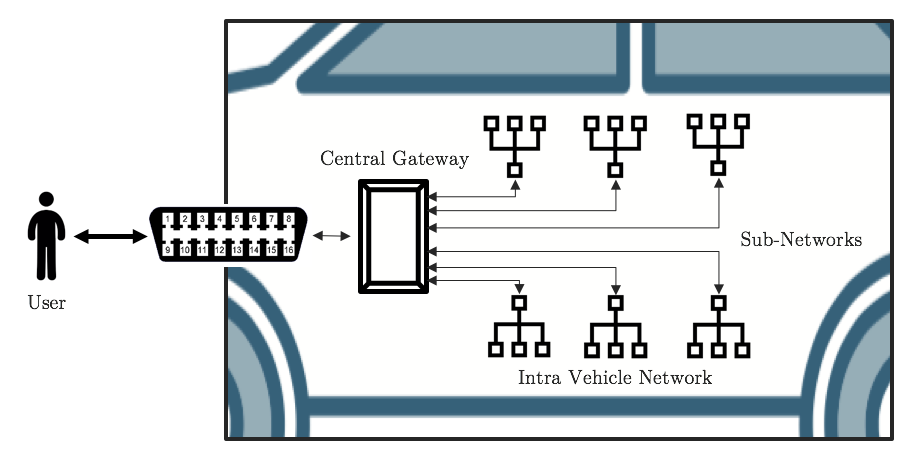
\includegraphics[width=\textwidth]{obd_topography.png}
	\caption{OBD-II System Topography.}
\end{figure}
 

\section{Challenges} \label{sec:challenges}
The main challenge of this research topic is to introduce a solution that ports well to the kind of hardware that is found in vehicles. Introducing new components into the internal vehicle network would surely simplify things. If this were the case, the solution could consist of introducing a small component that acts as a firewall for the OBD-II interface. However this implies that any potential real-world implementation requires the installation of this component into millions of currently in-use vehicles. Which, being a very costly endeavour, would deter any manufacturers from doing so. Therefore, a software-based approach is preferable. It is easy to deploy such a solution on extant cars, without requiring hardware modifications or excessive expenses. However, This approach introduces it's own challenges; namely, the limitations of ECU micro controllers. Indeed, any solution that isn't portable to a typical vehicle network because of memory limitations, limited processing power, incompatible architectures, etc., is ultimately rendered useless. It is worth noting that the solution proposed here is not intended to (and will not) protect against attacks using other attack vectors (e.g. TPMS, Bluetooth, etc.). This also applies to physical attacks. Indeed, any attacker gaining physical access to the vehicle has to ability to directly interface with the vehicle network (e.g. by physically tapping into the CAN bus). Typically, only the owner of the vehicle has this privilege, and it is safe to assume this person is reluctant to compromise the safety of their own vehicle. Unauthorised physical access should be mitigated by different means (e.g. car alarms, safe RKE systems, the authorities, etc.). The main challenges of this thesis paper are summarized as follows:

\begin{itemize}
	\item \textbf{portability:} The solution should port well to existing vehicle networks. 
	\item \textbf{Speed:} The solution should not impede the operation of other processes running on the same network.
	\item \textbf{Security:} The solution should be sufficiently secure according to current computer safety standards. 
\end{itemize}

\section{Contribution}
\label{sec:contributions}

The contribution of this thesis can be summarized as follows:

\begin{itemize}
	\item Overcoming the security limitation identified by the unauthorised access to the vehicle CAN network via the OBD-II port, by designing and developing a role-based access control model based on public key cryptography.
	
	\item Providing an open source proof of concept implementation of our designed model on a CAN-enabled resource-constrained ECU that is used in various automotive models \cite{Michel}. Furthermore, we evaluate and show that our approach is secure, feasible and lightweight in terms of memory footprint and runtime overhead.
\end{itemize} 

\section{Text Outline}
The remainder of this text is separated into five chapters:
\begin{itemize}
	\item \textbf{Chapter \ref{chap:background}} starts with a discussion of the design of intra vehicle networks. In lieu with this intention, the CAN protocol and the OBD-II standard are presented in detail. The second part of this chapter is a technical primer to all the security systems that are applied in our proposed solution. The main takeaway of this chapter consists of a solid technical background, allowing the reader to correctly interpret the rest of this paper.
	
	\item \textbf{Chapter \ref{chap:related_work}} is a survey of several studies that are topically related to this paper. The idea is that this will help to contextually situate our study, as well as getting the reader up to date with the current state of affairs vis-\`a-vis automotive network security.
	
	\item \textbf{Chapter \ref{chap:solution}} illustrates the main research topic of this paper. Namely, the vulnerability of the OBD-II interface. A detailed discussion of this problem is held, illustrated by some example attacks. A suitable attacker model is also defined. In the last section of this chapter our proposed solution is presented, namely OBD-II role-based access control. A detailed description of the design is given, accompanied by a series of diagrams.
	
	\item \textbf{Chapter \ref{chap:implementation}} describes a demo implementation of our solution. Where two microcontrollers are programmed to perform the authentication procedures introduced in Chapter \ref{chap:solution}. Furthermore, this implementation is evaluated in terms of portability, speed and security.
	
	\item \textbf{Chapter \ref{chap:conclusion}} Reviews the contributions of this thesis paper with respect to the results of the evaluation performed in Chapter \ref{chap:implementation}. We also present a series of future research topics introduced by our proposed solution.
\end{itemize}